\clearpage
\sffamily
{\bfseries\color[rgb]{0.4,0.4,0.4}
Law 1 -- The Field of Play}
\phantomsection
\addcontentsline{toc}{section}{Law 1 -- The Field of Play}

\bigskip
{\bfseries Field surface}

\headlinebox
 
Matches may be played on artificial surfaces with a height of approximately 30 mm.

\greyed{
(replaces: Matches may be played on natural or artificial surfaces, according to the rules of the competition.)}


\bigskip

{\sffamily
The colour of artificial surfaces must be green. }




\greyed{\bigskip
(suspended: Where artificial surfaces are used in either competition matches between representative teams of member associations affiliated to FIFA or international club competition matches, the surface must meet the requirements of the FIFA Quality Concept for Football Turf or the International Artificial Turf Standard, unless special dispensation is given by FIFA.) }


\bigskip

{\bfseries
Field markings}

\headlinebox

The field of play must be rectangular and marked with lines. These lines belong to the areas of which they are boundaries.

\bigskip

The two longer boundary lines are called touch lines. The two shorter lines are called goal lines.

\bigskip

The field of play is divided into two halves by a halfway line, which joins the midpoints of the two touch lines.

\bigskip

The centre mark is indicated at the midpoint of the halfway line. A circle with a radius of 0.75 m is marked around it.
\greyed{(replaces: A circle with a radius of 9.15 m (10 yds) is marked around it.)}



\greyed{\bigskip
(suspended: Marks may be made off the field of play, 9.15 m (10 yds) from the corner arc and at right angles to the goal lines and the touch lines, to ensure that defending players retreat this distance when a corner kick is being taken.) }

\bigskip

{\textbf{Dimensions}}

\headlinebox

The length of the touch line must be greater than the length of the goal line. 

\bigskip

\begin{tabular}{lll}
Length (touch line): &approximately &9 m \\
Width (goal line): &approximately &6 m
\end{tabular}

\greyed{
(replaces:

\begin{tabular}{lll}
Length (touch line): &minimum &90 m \\
&maximum &120 m \\
Width (goal line): &minimum &45 m \\
&maximum &90 m)
\end{tabular}
}

\bigskip

All lines must be of the same width, which must be approximately 5 cm. 

\greyed{
(replaces: All lines must be of the same width, which must be not more than 12 cm (5 ins).)}


\bigskip

International matches 

\begin{tabular}{lll}
Length (touch line): &approximately &9 m \\
Width (goal line): &approximately &6 m
\end{tabular}

\greyed{
(replaces: 

\begin{tabular}{lll}
Length (touch line): &minimum &100 m \\
&maximum &110 m \\
Width (goal line): &minimum &64 m \\
&maximum &75 m)
\end{tabular}
}

\bigskip

{\bfseries The goal area }

\headlinebox

Two lines are drawn at right angles to the goal line, \textcolor{blue}{\sout{1.6 m for KidSize and}} 1.2 m \textcolor{blue}{\sout{for TeenSize and AdultSize}} from the inside of each goalpost. These lines extend into the field of play for a distance of 1 m and are joined by a line drawn parallel with the goal line. The area bounded by these lines and the goal line is the goal area. 

\greyed{
(replaces: Two lines are drawn at right angles to the goal line, 5.5 m (6 yds) from the inside of each goalpost. These lines extend into the field of play for a distance of 5.5 m (6 yds) and are joined by a line drawn parallel with the goal line. The area bounded by these lines and
the goal line is the goal area. )}

\bigskip

{\bfseries The penalty area }

\headlinebox

\greyed{
(suspended: Two lines are drawn at right angles to the goal line, 16.5 m (18 yds) from the inside of each goalpost. These lines extend into the field of play for a distance of 16.5 m (18 yds) and are joined by a line drawn parallel with the goal line. The area bounded by these lines and the goal line is the penalty area.) \bigskip}



A penalty mark is made 2.1 m from the midpoint between the goalposts and equidistant to them. 
\greyed{(replaces: Within each penalty area, a penalty mark is made 11 m (12 yds) from the midpoint between the goalposts and equidistant to them.)\bigskip}



\greyed{
(suspended: An arc of a circle with a radius of 9.15 m (10 yds) from the center of each penalty mark is drawn outside the penalty area.)}

\simplify{
\bigskip

{\textbf{Flagposts} }

\headlinebox

\greyed{
(suspended: A flagpost, not less than 1.5 m (5 ft) high, with a non-pointed top and a flag must be placed at each corner.) }

\bigskip

\greyed{
(suspended: Flagposts may also be placed at each end of the halfway line, not less than 1 m (1 yd) outside the touch line.)}

\bigskip

{\bfseries The corner arc }

\headlinebox

\greyed{
(suspended: A quarter circle with a radius of 1 m (1 yd) from each corner flagpost is drawn inside the field of play.)}
}

\bigskip

{\bfseries Goals }

\headlinebox

A goal must be placed on the center of each goal line.


\bigskip

A goal consists of two upright posts equidistant from the corner flagposts and joined at the top by a horizontal crossbar. The goalposts and crossbar must be made of wood, metal or other approved material. They must be square, rectangular, round or elliptical in shape and must
not be dangerous to players.

\bigskip

The distance between the posts is \textcolor{blue}{\sout{1.8 m for KidSize and}} 2.6 m \textcolor{blue}{\sout{for TeenSize and AdultSize}} and the distance from the lower edge of the crossbar to the ground is \textcolor{blue}{\sout{1.1 m for KidSize and}} 1.8 m \textcolor{blue}{\sout{for TeenSize and AdultSize}}. 

\greyed{
(replaces: The distance between the posts is 7.32 m (8 yds) and the distance from the lower edge of the crossbar to the ground is 2.44 m (8 ft).)}

\bigskip

\greyed{
(suspended: figures of different goal post geometries)}

\bigskip

\greyed{
(suspended: The position of the goalposts in relation to the goal line must be according to the graphics below.)}

\bigskip

If the shape of the goalposts is square (viewed from above), the sides must be parallel or perpendicular to the goal line. The sides of the crossbar must be parallel or perpendicular to the field plane.

\bigskip

If the shape of the goalposts is elliptical (viewed from above), the longest axis must be perpendicular to the goal line. The longest axis of the crossbar must be parallel to the field plane.

\bigskip

If the shape of the goalposts is rectangular (viewed from above), the longest side must be perpendicular to the goal line. The longest side of the crossbar must be parallel to the field plane.

\bigskip

Both goalposts and the crossbar have the same width and depth, \textcolor{magenta}{which do not exceed 12 cm (5 ins).} 
The goal lines must be approximately 5 cm of width. 
\greyed{
(replaces: The goal lines must be of the same width as the goalposts and the crossbar.)} 
Nets (new:) \textcolor{magenta}{which must not be green or white} may be attached to the goals and the ground behind the goal, provided that they are properly supported and do not interfere with the goalkeeper. 

\bigskip

The goalposts and crossbars must be white.

\bigskip

{\bfseries Safety}

\headlinebox

Goals must be anchored securely to the ground. Portable goals may only be used if they satisfy this requirement.

\bigskip

{\bfseries The field of play}

\headlinebox 

\begin{center}
\begin{figure}[h]
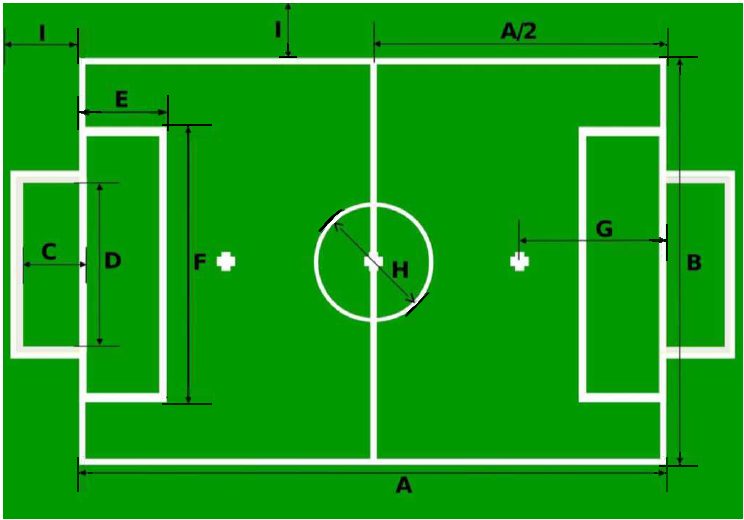
\includegraphics[width=\textwidth]{img/field.png}
\caption{Humanoid robot soccer field (not to scale)}
\end{figure}
\end{center}
\newpage

\begin{center}
\tablehead{}
\begin{table}[h]
\caption{Approximate dimensions of the rectangular field of soccer play.}
\centering
\begin{tabular}{|l|l|c|}
\hline
A & Field length & 9 m\\
\hline
B & Field width &  6 m\\
\hline
C & Goal depth & \textcolor{magenta}{0.6 m}\\
\hline
D & Goal width & \textcolor{magenta}{2.6 m}\\
\hline
~ & Goal height & \textcolor{magenta}{1.8 m}\\
\hline
E & Goal area length & 1 m\\
\hline
F & Goal area width & 5 m\\
\hline
G & Penalty mark distance & 2.1 m\\
\hline
H & Center circle diameter & 1.5 m\\
\hline
I & Border strip width (min.) & 0.7 m\\
\hline
\end{tabular}
\end{table}
\end{center}

\greyed{
(replaces figure of field)}

\simplify{
\bigskip

{\bfseries Corner flagpost}

\headlinebox 

\greyed{(suspended: figure of flagpost)}

\bigskip

{\bfseries Metric measurements}

\headlinebox 

\greyed{(suspended: figure with metric dimensions of field)}

\bigskip

{\bfseries Imperial measurements}

\headlinebox 

\greyed{(suspended: figure with imperial dimensions of field)}
}

\simplify{
\clearpage

{\bfseries Decisions of the International F.A. Board}

\headlinebox 

\greyed{
(suspended: Decision 1

Where a technical area exists, it must meet the requirements approved by the International F.A. Board, which are contained in the section of this publication entitled The Technical Area.)}

\bigskip

\greyed{
(suspended: Decision 2

Where goal-line technology (GLT) is used, modifications to the goal frame may be allowed. They must be in accordance with the specifications stipulated in the FIFA Quality Programme for GLT and according to the above description, ``Goals''.) }
}
